
\begin{figure*}[t]
\centering
\subfigure{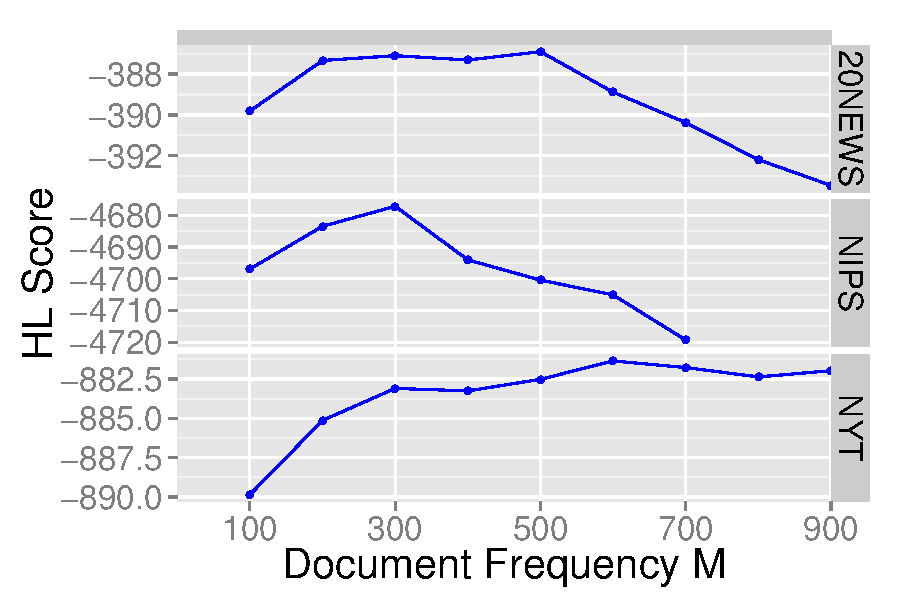
\includegraphics[width=0.48\linewidth]{2014_acl_reganchor/figures/M_HL.pdf}}
\subfigure{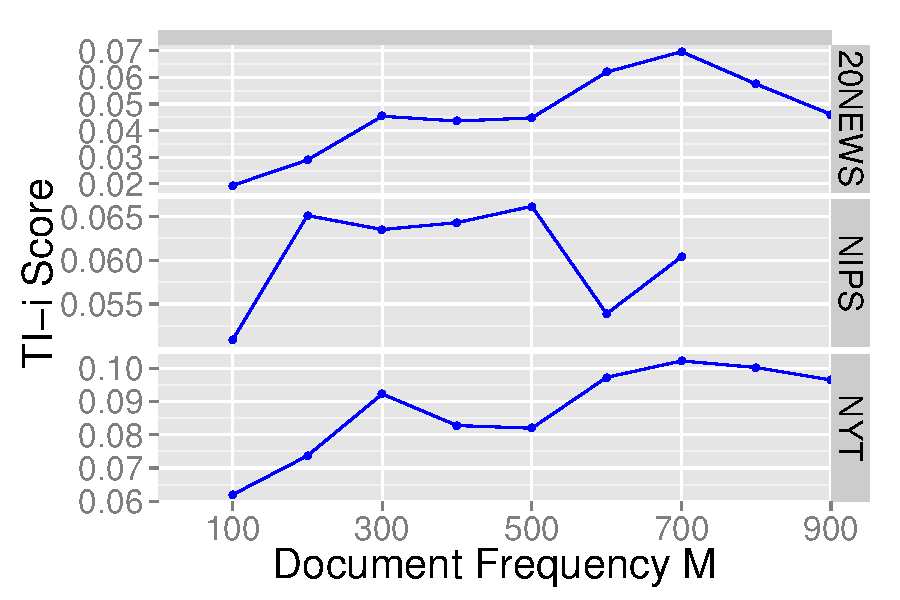
\includegraphics[width=0.48\linewidth]{2014_acl_reganchor/figures/M_TI.pdf}}
\caption{Grid search for document frequency $M$ for our datasets with
  20 topics (other configurations not shown) on development data. The
  performance on both \abr{hl} and \abr{ti} score indicate that the
  unregularized {\bf anchor} algorithm is very sensitive to $M$.  The
  $M$ selected here is applied to subsequent models.}
\label{fig:anchor-select}
\end{figure*}



\section{Regularization Improves Topic Models}
\label{sec:experiments}

In this section, we measure the performance of our proposed
regularized anchor word algorithms.  We will refer to specific
algorithms in bold.  For example, the original anchor algorithm is
{\bf anchor}.  Our $L_2$ regularized variant is {\bf anchor-$L_2$},
and our beta regularized variant is {\bf anchor-beta}.  To provide
conventional baselines, we also compare our methods against topic
models from variational inference \cite[{\bf
  variational}]{blei-03} and \abr{mcmc}~\cite[{\bf
  \abr{mcmc}}]{griffiths-04,mallet}.

We apply these inference strategies on three diverse corpora:
scientific articles from the Neural Information Processing
Society~(\abr{nips}),\footnote{\url{http://cs.nyu.edu/~roweis/data.html}} Internet newsgroups
postings~(\abr{20news}),\footnote{\url{http://qwone.com/~jason/20Newsgroups/}} and New York Times
editorials~\cite[\abr{nyt}]{sandhaus-08}.  Statistics for the datasets
are summarized in Table~\ref{tab:corpus}.  We split each dataset into
a training fold (70\%), development fold (15\%), and a test
fold (15\%): the training data are used to fit models; the development
set are used to select parameters (anchor threshold $M$, document
prior $\alpha$, regularization weight $\lambda$); and final results
are reported on the test fold.

We use two evaluation measures, held-out likelihood \cite[{\bf
  \abr{hl}}]{blei-03} and topic interpretability~\cite[{\bf
  \abr{ti}}]{chang-09b,newman-10}.  Held-out likelihood measures how
well the model can reconstruct held-out documents that the model has
never seen before.  This is the typical evaluation for probabilistic
models.  Topic interpretability is a more recent metric to capture how
useful the topics can be to human users attempting to make sense of a
large datasets.

Held-out likelihood cannot be computed with existing {\bf anchor} algorithms, so
we use the topic distributions learned from {\bf anchor} as input to a reference variational
inference implementation~\cite{blei-03} to compute {\bf \abr{hl}}.
This requires an additional parameter, the Dirichlet prior
$\alpha$ for the per-document distribution over topics.  We select $\alpha$
using grid search on the development set.

To compute {\bf \abr{ti}} and evaluate topic coherence, we use normalized
pairwise mutual information~(\abr{npmi})~\cite{lau-14} over topics' twenty most
probable words.  Topic coherence is computed against the \abr{npmi} of a
reference corpus.  For coherence evaluations, we use both intrinsic and
extrinsic text collections to compute \abr{npmi}.  Intrinsic coherence
(\abr{ti}-i) is computed on training and development data at development time
and on training and test data at test time.
Extrinsic coherence (\abr{ti}-e) is computed from
English Wikipedia articles, with disjoint halves (1.1 million pages each) for distinct
development and testing \abr{ti}-e evaluation.


\begin{figure*}[t!]
\centering
\subfigure{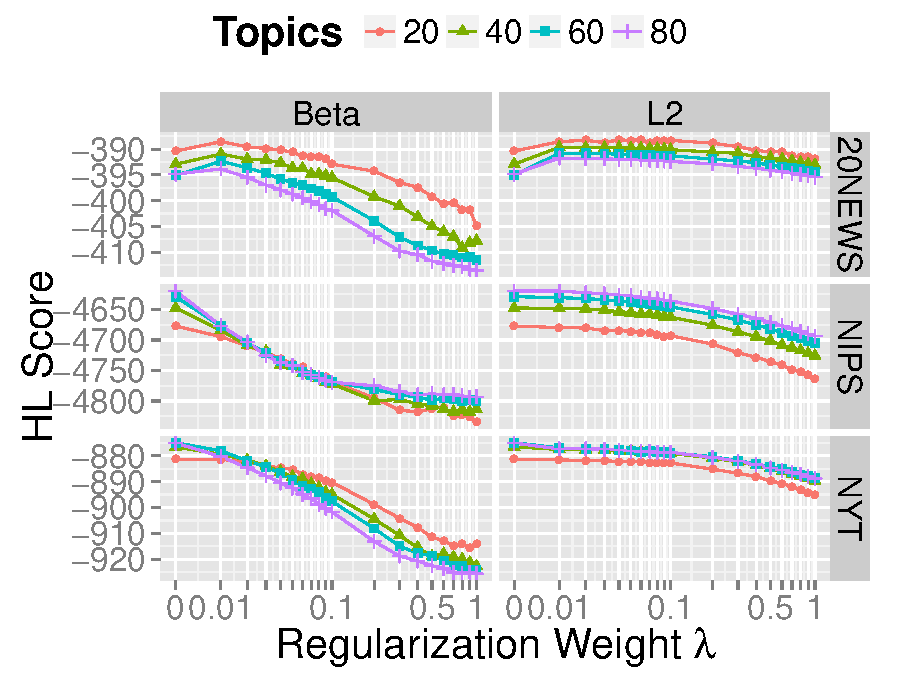
\includegraphics[width=0.48\linewidth]{2014_acl_reganchor/figures/HL_HL.pdf}}
\subfigure{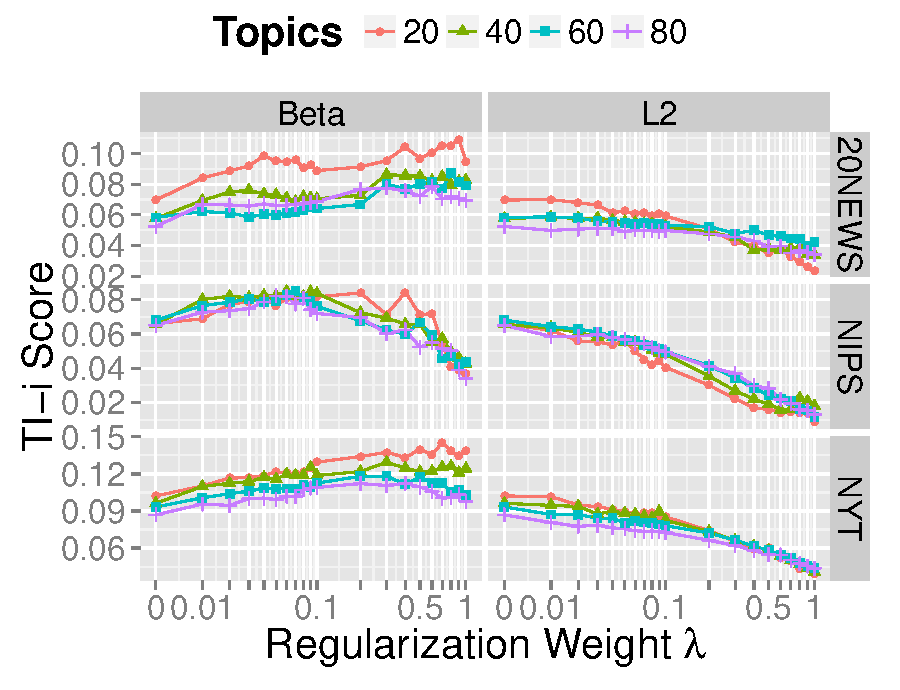
\includegraphics[width=0.48\linewidth]{2014_acl_reganchor/figures/TI_TI.pdf}}
\caption{Selection of $\lambda$ based on \abr{hl} and \abr{ti}
  scores on the development set. The value of $\lambda =0$ is equivalent to the original {\bf
    anchor} algorithm; regularized versions find better solutions as
  the regularization weight $\lambda$ becomes non-zero.}
\label{fig:select-lambda}
\end{figure*}


\subsection{Grid Search for Parameters on Development Set}
\label{sec:parameter-search}

\paragraph{Anchor Threshold}

A good anchor word must have a unique, specific context but also
explain other words well.  A word that appears only once will have a
very specific cooccurence pattern but will explain other words'
coocurrence poorly because the observations are so
sparse.  As discussed in Section~\ref{sec:anchor}, the {\bf anchor}
method uses document frequency $M$ as a threshold to only consider
words with robust counts.

Because all regularizations benefit equally from higher-quality anchor
words, we use cross-validation to select the document frequency cutoff
$M$ using the unregularized {\bf anchor} algorithm.
Figure~\ref{fig:anchor-select} shows the performance of {\bf anchor}
with different $M$ on our three datasets with 20 topics for our two
measures \abr{hl} and \abr{ti}-i.

\paragraph{Regularization Weight}

Once we select a cutoff $M$ for each combination of dataset,
number of topics $K$ and a evaluation measure, we select a regularization weight
$\lambda$ on the development set.  Figure~\ref{fig:select-lambda}
shows that {\bf beta} regularization framework improves topic
interpretability \abr{ti}-i on all datasets and improved the held-out
likelihood \abr{hl} on \abr{20news}.  The $L_2$ regularization also
improves held-out likelihood \abr{hl}
 for the \abr{20news} corpus (Figure~\ref{fig:select-lambda}).

In the interests of space, we do not show the figures for selecting $M$
 and $\lambda$ using \abr{ti}-e, which is similar to \abr{ti}-i: {\bf
   anchor-beta} improves \abr{ti}-e score on all datasets, {\bf
   anchor-$L_2$} improves \abr{ti}-e on \abr{20news} and \abr{nips}
 with 20 topics and \abr{nyt} with 40 topics.

\subsection{Evaluating Regularization}

With document frequency $M$ and regularization weight $\lambda$
selected from the development set, we compare the performance of those
models on the test set.  We also compare with standard implementations
of Latent Dirichlet Allocation: Blei's \abr{ldac} ({\bf variational}) and
Mallet ({\bf mcmc}).  We run 100 iterations for \abr{ldac} and 5000
iterations for Mallet.

Each result is averaged over three random runs and appears in
Figure~\ref{fig:results}.  The highly-tuned, widely-used implementations
uniformly have better held-out likelihood than {\bf anchor}-based methods, but
the much faster {\bf anchor} methods are often comparable.  Within {\bf
  anchor}-based methods, $L_2$-regularization offers comparable held-out
likelihood as unregularized {\bf anchor}, while {\bf anchor-beta} often has
better interpretability.  Because of the mismatch between the specialized
vocabulary of \abr{nips} and the general-purpose language of Wikipedia,
\abr{ti}-e has a high variance.

\begin{figure*}[t]
\centering
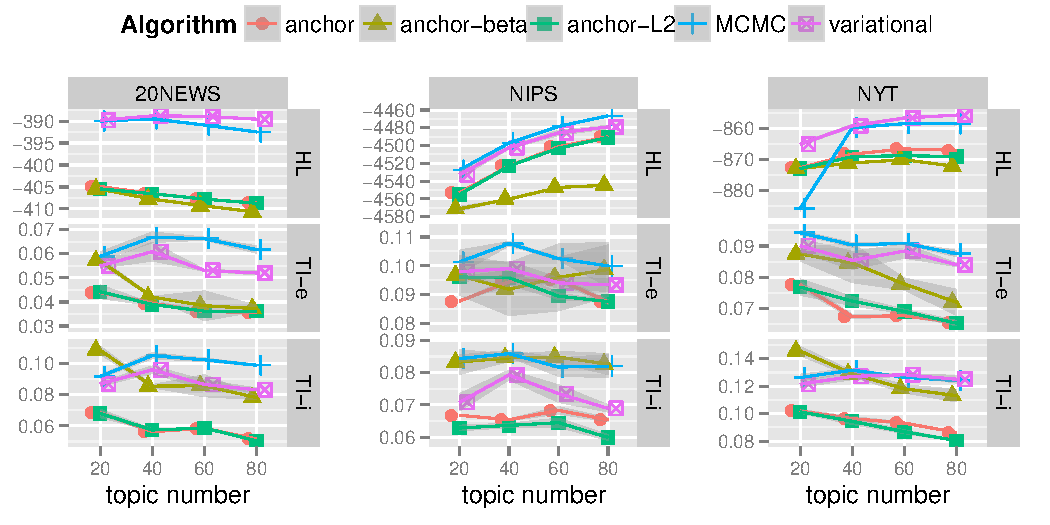
\includegraphics[width=\linewidth]{2014_acl_reganchor/figures/results_option3}
\caption{Comparing {\bf anchor-beta} and {\bf anchor-$L_2$} against
  the original {\bf anchor} and the traditional {\bf variational} and
  {\bf MCMC} on \abr{hl} score and \abr{ti} score.  {\bf variational}
  and {\bf mcmc} provide the best held-out generalization.  {\bf
    anchor-beta} sometimes gives the best \abr{ti} score and is
  consistently better than {\bf anchor}.  The specialized vocabulary
  of \abr{nips} causes high variance for the extrinsic
  interpretability evaluation (\abr{ti}-e).}
\label{fig:results}
\end{figure*}

\begin{table*}[t!]
\begin{small}
   \begin{center}

\begin{tabular}{|p{1cm}|c|p{8cm}|} \hline
Topic & Shared Words & Original (Top, green) vs. Informed $L_2$ (Bottom, orange) \\ \hline
\multirow{2}{*}{soviet}	&	\multirow{2}{5cm}{american make president {\bf soviet} union {\bf war} years } &	\cellcolor{green!30}gorbachev moscow russian force economic world europe political communist lead reform germany country \\&	&	\cellcolor{orange!30}{\bf military} state {\bf service} washington \red{bush} {\bf army} unite {\bf chief} {\bf troops} {\bf officer} \red{nuclear} time week \\ \hline
\multirow{2}{*}{district}	&	\multirow{2}{5cm}{{\bf assembly} board city {\bf county} {\bf district} {\bf member} state york } &	\cellcolor{green!30}representative manhattan brooklyn queens election bronx council island local incumbent housing municipal \\&	&	\cellcolor{orange!30}{\bf people} {\bf party} {\bf group} {\bf social} \red{republican} year make years {\bf friend} \red{vote} {\bf compromise} million \\ \hline
\multirow{2}{*}{peace}	&	\multirow{2}{5cm}{american force government israel {\bf peace} political president state unite washington } &	\cellcolor{green!30}war military country minister leaders nation world palestinian israeli election \\&	&	\cellcolor{orange!30}{\bf offer} {\bf justice} {\bf aid} {\bf deserve} make \red{bush} years {\bf fair} \red{clinton} {\bf hand} \\ \hline
\end{tabular}
\begin{tabular}{|p{1cm}|c|p{7cm}|} \hline
\multirow{2}{*}{arms}	&	\multirow{2}{6cm}{{\bf arms} bush congress force iraq make north nuclear president state washington weapon } &	\cellcolor{green!30}administration treaty missile defense war military korea reagan \\&	&	\cellcolor{orange!30}{\bf agree} {\bf agreement} american {\bf accept} unite {\bf share} \red{clinton} years \\ \hline
\multirow{2}{*}{trade}	&	\multirow{2}{6cm}{{\bf administration} america american country {\bf economic} government make president state {\bf trade} unite washington } &	\cellcolor{green!30}world market japan foreign china policy price political \\&	&	\cellcolor{orange!30}{\bf business} {\bf economy} \red{congress} year years \red{clinton} \red{bush} {\bf buy} \\ \hline
\end{tabular}

   \end{center}
\end{small}
\caption{Examples of topic comparison between {\bf anchor} and informed {\bf
    anchor-$L_2$}. A topic is labeled with the anchor word for that topic. The
  {\bf bold} words are the informed prior from \abr{liwc}. With an informed
  prior, relevant words appear in the top words of a topic; this also draws
  in other related terms (red). }
\label{tab:compare-informed}
\end{table*}

\subsection{Informed Regularization}
\label{sec:informed}

A frequent use of priors is to add information to a model.  This is not possible
with the existing {\bf anchor} method.  An informed prior for topic models seeds
a topic with words that describe a topic of interest.  In a topic model, these
seeds will serve as a ``magnet'', attracting similar words to the
topic~\cite{zhai-12}.

We can achieve a similar goal with {\bf anchor-$L_2$}.  Instead of
encouraging anchor coefficients to be zero in
Equation~\ref{eq:anchorl2}, we can instead encourage word
probabilities to close to an arbitrary mean $\mu_{i,k}$.  This vector
can reflect expert knowledge.

One example of a source of expert knowledge is Linguistic Inquiry and Word
Count~\cite[\abr{liwc}]{pennebaker-99}, a dictionary of keywords related to
sixty-eight psychological concepts such as \underline{positive emotions},
\underline{negative emotions}, and \underline{death}.  For example, it
associates ``excessive, estate, money, cheap, expensive, living, profit, live,
rich, income, poor, etc." for the concept \underline{materialism}.

We associate each anchor word with its closest \abr{liwc} category based on
the cooccurrence matrix $\bm{Q}$. This is computed by greedily finding the
anchor word that has the highest cooccurrence score for any \abr{liwc} category:
we define the score of a category to anchor word $w_{s_k}$ as $\sum_i Q_{s_k, i}$,
where $i$ ranges over words in this category; we compute the scores of all categories to
all anchor words; then we find the highest score and assign the category to that anchor
word; we greedily repeat this process until all anchor words have a category.

Given these associations, we create a goal mean $\mu_{i,k}$.  If there
are $L_i$ anchor words associated with \abr{liwc} word $i$, $\mu_{i, k}
= \frac{1}{L_i}$ if this keyword $i$ is associated with anchor word
$w_{s_k}$ and zero otherwise.

We apply {\bf anchor-$L_2$} with informed priors on \abr{nyt}
with twenty topics and compared the topics against the
original topics from {\bf anchor}.  Table~\ref{tab:compare-informed}
shows that the topic with anchor word ``soviet'', when combined with
\abr{liwc}, draws in the new words
``bush'' and ``nuclear''; reflecting the threats of force during the
cold war.  For the topic with topic word ``arms'', when associated
with the \abr{liwc} category \underline{} with the terms ``agree'' and
``agreement'', draws in ``clinton'', who represented a more
conciliatory foreign policy compared to his republican predecessors.
